% Carleton University SCE 4th Year Project thesis style
% University of Ottawa MSc thesis style -- modifications to the report style
% modification of suthesis style of Stanford University
% Example of use:
\documentclass[12pt]{report}
\usepackage{setspace}
\doublespacing
\usepackage[margin=2.5cm]{geometry}
\usepackage{amsmath,amssymb,amsthm}
\usepackage[nottoc,numbib]{tocbibind}
\usepackage{graphicx}
%Forces figures to appear within a section, if more specific placement is needed go to:
% http://tex.stackexchange.com/questions/279/how-do-i-ensure-that-figures-appear-in-the-section-theyre-associated-with
\usepackage[section]{placeins}
\usepackage{SCE4YPTemplate}
\usepackage{url}
\usepackage[
	backend=bibtex,
	natbib=true,
	style=numeric,
	sorting=none
]{biblatex}
\usepackage[scientific-notation=true, binary-units=true]{siunitx}
\sisetup{per-mode=fraction}%
\sisetup{scientific-notation=false}%

\makeatletter
\def\blx@maxline{77}
\makeatother

\bibliography{report}

\begin{document}
\title{SYSC4907 Project: \\ Sensor-Based Access Control System}
\author{
    Craig Shorrocks,
    Jessica Morris,
    Richard Perryman
}
	    % Remember to use your titles
	    % Use \copyrightyear{1885} to force a particular year
	    % for the copyright statement.
\copyrightfalse % do not produce a separate copyright page
		    % otherwise use \copyrighttrue
%    \figurespagefalse % do not produce a separate figures page
%    \tablespagefalse  % do not produce a separate tables page

% Here you insert the stuff that comes before the preface
% Each preface section is contained in a \prefacesection and starts on a
% new page.  These are numbered using Roman numerals.
% If there are no such pages, do not remove the \beforepreface command
% since it creates the title page.
\beforepreface

%=================================================================================

\prefacesection{Abstract}
	This report tells you all you need to know about something.

%=================================================================================

\prefacesection{Acknowledgements}
	I would like to thank my supervisor, anyone who paid me money, gave me
	equipment, etc.
    % Supervisors
    % Jennifer Wolters, for giving us some free money
    % Nagui Mikhail, for soldering stuff for Jess
    % Michel and Normand Leroux, for their carpentry work on the demo unit

%=================================================================================

% For some reason, these seem to require that you run latex twice?

\prefaceTOC   % to print the Table of Contents
\listoffigures   % to print the List of Figures
\listoftables   % to print the List of Tables

%=================================================================================
		            
\prefacesection{List of Abbreviations}
    
\begin{tabular}[t]{l@{\hspace*{2cm}}l}
	AID & Application IDentifier \\
	APDU & Application Protocol Data Unit \\
	API & Application Programming Interface \\
	HMAC & Keyed-Hash Message Authentication Code \\
    IO & Input/Output \\
	JSON & JavaScript Object Notation \\
	MVC & Model-View-Controller \\
	NFC & Near Field Communication \\
	RFC & Request for Comments \\
\end{tabular}

%=================================================================================

\endpreface
	
%=================================================================================

\chapter{Introduction}

Give an introduction to your project.  This might include:
\begin{itemize}
  \item Motivation for your project
  \item Problem you are trying to solve
  \item Scope of your project
  \item Organization of your report
\end{itemize}
You should tune this appropriately for what best suits your project.


%=================================================================================

\chapter{The Engineering Project}

%=================================================================================

\section{Health and Safety}

The main health and safety concern for this project was ensuring the safe preparation of circuits for the hardware 
component. The change of bodily harm due to electric shock was possible, as the highest-risk component of the project 
drew $\SI{650}{\milli\ampere}$ of current at 12V direct current. Since $\SI{650}{\milli\ampere}$ is above the 
$\SI{500}{\milli\ampere}$ threshold for possible heart fibrillation~\autocite{CURRENTDANGER}, the following standards
were enforced to mitigate safety risks when handling the electrical components:
\begin{itemize}
    \item The workspace and components were kept dry at all times
    \item Participants ensured they were sufficiently grounded before handling components
    \item Ground pins were connected first, to ensure any charged components would discharge
    \item Components' wiring was not altered while the system was powered on
\end{itemize}
% J - ask if health and safety for construction of the demo unit is necessary here
% (it probably is)

%=================================================================================

\section{Engineering Professionalism}

Using their course experience of ECOR 4995 Professional Practice, students should demonstrate how their professional responsibilities were met by the goals of their project and/or during the performance of their project. 

%=================================================================================

\section{Project Management}

One of the goals of the engineering project is real experience in working on a long-term team project.  Students should explain what project management techniques or processes were used to coordinate, manage and perform their project.

%=================================================================================

\section{Individual Contributions}

This section should carefully itemize the individual contributions of each team member. Project contributions should identify which components of work were done by each individual.  Report contributions should list the author of each major section of this report.

%---------------------------------------------------------------------------------

\subsection{Project Contributions}

Give the individual contributions of the each team member towards the project.

%---------------------------------------------------------------------------------

\subsection{Report Contributions}

Give the individual contributions of the each team member towards writing the
final report.

%=================================================================================

% Consider adding Node, Android? Maybe others?
\chapter{Technical Background}

%=================================================================================

\section{NFC}

%=================================================================================

\section{Cloud Computing}

%=================================================================================

%---------------------------------------------------------------------------------

\subsection{AWS}

%=================================================================================

\section{Security}

%=================================================================================

\section{Single-Board Computers and Microcontrollers}

Insert blurb about what is a single-board thingamabob

%---------------------------------------------------------------------------------

\subsection{Raspberry Pi}

The Raspberry Pi is a credit-card-sized, single-board computer developed by the Raspberry Pi Foundation. In its initial 
design, it was intended to be a learning tool to introduce computer science to students at the pre-university  
level. However, its accessible price gave it increased appeal among hobby electronics enthusiasts, and it is now often 
used for robotics projects, media streaming, IoT projects, and more. Today, the Raspberry Pi has sold over ten million 
units [CITATION], with models ranging from the 5 USD Raspberry Pi Zero, to the 35 USD Raspberry Pi 3 Model B.
% One more paragraph here

%---------------------------------------------------------------------------------

\subsection{Arduino}



%=================================================================================

\chapter{Business Use Cases}

Design for our system began with considering use cases that could be handled by our system. This way, we could be sure
to only design features that would prove useful to some potential users, while also making sure that we don't miss any
features that are necessary. These use cases would also provide benefit to demonstrating our system, in that stepping
through a sample use case would show the value of the system to people without them requiring a strong technical
background.

We primarily focused on the four use cases that follow. These were outlined in our initial proposal and have remained
largely unchanged since then. They draw inspiration from situations that we either encountered ourselves or found
through common knowledge and research. Online shopping seemed like a ripe market for technology like the SBACS, and
mail delivery seemed that it followed a fairly similar system. Long term storage facilities also seemed as though they
would benefit from abstracting away the idea of keys. Once we had considered these use cases, we found that several of
the problems that they shared could be solved by a company which provided SBACS as a service.

%=================================================================================

\section{Online Order Secure Pickup}

With online shopping becoming more popular [], the hassle of being physically present to shop in stores 
could be eliminated by allowing customers to make an order and payment online, then pick up their products at the store 
using a SBACS-secured storage container. After a customer's order has been confirmed by the store to be packed 
and ready for pick-up, a store employee could create a link between their customer and the storage container that holds
that user's purchases. When the customer arrives at the store to pick up their items, 
they can gain access to the storage container assigned to them by using the authentication methods that they had
previously provided as the components of their identity. Once the customer has provided these authentication units
correctly, the link between their identity and the storage container is broken. This way, the user won't be able to
inappropriately access the storage container again, and a new link could be made for a different customer.

\begin{figure}
	\includegraphics[width=\textwidth]{Diagrams/Use-Case-Diagrams/online-order-secure-pickup-use-case-diagram}
	\caption{Online Order Secure Pickup Use Case Diagram}
	\label{fig:online-order-secure-pickup-use-case}
\end{figure}

A strong advantage of this system over existing ones, such as Walmart's Grab \& Go, is that it creates a digital 
fingerprint using a combination of authentication methods supported by the SBACS, which is more difficult to 
break via brute force than a 6-digit PIN []. In addition, with the entire process of shopping being 
expedited, customers will spend less time in stores and parking lots, leading to less congestion due to vehicle 
traffic. This system will also grant customers with mobility or vision impairments increased personal autonomy, as 
they will be able to retrieve their goods with less aid from store employees than traditional shopping allows. Customers
with impairments can perform their shopping online using their accessibility software, such as text-to-speech, instead 
of calling the store to request that an employee retrieve their goods. When the customer receives confirmation of their 
order and authentication tokens, they can access their assigned SBACS-secured locker in the store themselves, using 
their usual aids instead of occupying a store employee's time.

%=================================================================================

\section{Central Mail Package Pickup}

%=================================================================================

\section{Long Term Storage}

%=================================================================================

\section{Service Provider}

%=================================================================================

\chapter{Problem Analysis and System Design}

%=================================================================================

\section{Overall System Analysis}

The requirements of our system from the use cases described above lead us to a simple outline for the entire system.
The main component of the system would be the cloud server, which would store information regarding users, locks, and
the relationships between them. The lock hardware would need to be able to securely accept data from the user, and
securely send that data to the server for verification. Since handling electronic security can be difficult to do
manually, having an application that handles much of the busy work would greatly help users interact with the system.

% Not sure if this belongs here
One of the main goals of the system was to improve the reusability of the electronic keys that are created. For this
reason, the idea of a key was split into two parts: an authenticator, and an identity. Users would be able to create
many authenticators, which were things like a password, or a PIN. These then could be combined into an identity, which
would be used to open a particular lock. This allowed making identies that reuse the same authenticator, and reusing
identities for different locks.

Another goal of the system was to provide additional behaviour on top of just being able to unlock particular locks.
This extra behaviour was captured in the notion of a registration, which ties one lock to one identity. Through the
registration, we were able to implement notifications to the user as well as streaming of the lock's contents.

% Add picture of database stuff?

%=================================================================================

\section{NFC}

Determining how NFC communication should take place required analysis of two hardware systems: NFC card readers, as well
as mobile devices. The most desirable protocol would be able to handle the widest variety of available hardwares for
the two devices. The performance considerations between modes was fairly minimal, so preference was placed on the
portability of the solution.

%---------------------------------------------------------------------------------

\subsection{Card Readers}

% Todo: sources
Since NFC cards are primarily designed for NFC communications, there were few restrictions that stemmed from potential
choices in card reader. Since NFC communications are specified by the ISO, most cards support enough protocols that any
decision on our part would be very likely to be supported by any card that would be desirable for any other reason.

%---------------------------------------------------------------------------------

\subsection{Mobile Devices}

The two most popular operating systems for mobile devices are iOS and Android []. Since iOS devices have NFC disabled
for everything except Apple Pay[], the only option that remained was Android. Apple devices would represent a large
part of the potential market, so alternatives to NFC would have to be considered.

Among Android devices, there exist devices which have hardware support for NFC communications, and those which rely on
host-based card emulation. Devices with hardware support have a component called a Secure Element which performs all of
the communication with the external NFC terminal. Later, applications can query this element to determine the status of
the transaction, as well as other data. Devices which use host-based card emulation use a software implementation of
secure elements. Since host-based card emulation is done through software, it will run on all Android devices running
version 4.4 or greater[], which represents over 99\% of all devices currently in use.

% Find out which protocol we actually use!
Android offers an API called Beam which is the only way Anndroid devices can use NFC in active mode []. Beam,
however, does not support sending more than one message between devices. Since the information we are sending can be
fairly large in the interest of security, this was not feasible given the restrictions of the NFC protocols we used.
Further, active communications are easier to eavesdrop on, as discussed in the background section. We decided that these
costs outweighed the simplicity of the Beam API, so passive communications were chosen for the implementation.

% Discuss AID here? or in implementation? Here for now I guess
Since more than one application could potentially want to handle an NFC message, the message protocol contains a field
called the Application IDentifier, or AID []. These AIDs are just large numbers which identify which application should
handle the associated message. The Android operating system is responsible for delivering the APDUs to the
appropriate application's service []. Reserving a particular AID costs money, so we decided that the probability of a
collision ocurring when taking a public AID would be an acceptable cost for the purpose of our demonstrative
implementation.

%---------------------------------------------------------------------------------

\subsection{Protocol}

Since our NFC communications may require more data than can be fit within an Application Protocol Data Units (APDUs), we
required a protocol which would handle segmenting and recombining the message. APDUs are defined in ISO 7816-4 [] and are
the units used by ISO 14443-4 [], which describes the transmission protocol used by NFC devices. They are restricted to
256 bytes, including headers.

% Todo, some fact checking
To work around this, the hardware device connected to the shield maintains a buffer. Under ISO 14443-4, messages can be
reliably transferred, so managing this buffer is the main consideration of our protocol. The hardware determines the
maximum amount of data that can be stored in one APDU, and fills in this value into the length field of the APDU that it
sends to the Android device. Then, the Android application responds with the minimum of that much data,  and all of the
remaining data that it has to send. Once the hardware receives an amonut of data less than the potential maximum, it
deactivates the connection. In the event that the data from the Android application fits exactly into the last message
that would be sent, the protocol still works, as the application will then respond with zero data bytes.

% Todo: MSC / FSMs?

%=================================================================================

\section{Android}

The Android application's goal was to provide the end users with an easy way of interacting with the SBACS system.
Therefore the application was designed to be as simple as possible while still maintaining flexibility when dealing with
the cloud server as well as the many potential hardware devices.

%---------------------------------------------------------------------------------

\subsection{User Interface}

The natural decision for designing the basic workings of the application was to use the Model-View-Controller (MVC) 
design pattern. This pattern separates the underlying data (model) from the display that the user sees (view) as well as
the components that the user interacts with (controller). Android provides APIs to support MVC. Model objects can be
simple objects, but view objects can subclass the View class or its more specific subclasses, and the controller
objects can subclass the Adapter class or its subclasses.

Android applications themselves should follow the patterns set out by the standards. Activity classes represent the
pages that contain the various views and controllers that users can interact with. We decided on a design where the user
first encouters a login Activity, which prompts them to either sign up or log in. Once the user has logged in, we
provide a hub Activity which leads to the various other Activities in the application. These other Activities show the
various data related to the user, such as their authenticators and identities.

Communication between Activities is handled by a class provided by Android called an Intent. Intent objects contain
information about the nature of the request to begin the new Activity. In this way, information such as the user's
identification number could be sent from the login Activity to the hub Activity, which would allow the application to
correctly load the information from that user when displaying the data Activities.

%---------------------------------------------------------------------------------

\subsection{Notifications}

The design for the notifications that would inform end users of information such as their newly available registration
with a particular lock was based partly on decreasing load on the server. Having the server maintain a large amount of
session information as well as spending time and memory on the timers to be able to update the user of these changes
was thought to be too great a cost. For this reason, it seemed simpler and more effective to have the application poll
the server at a particular access point for new information.

This polling was implemented simply in the application using a service which runs in the background of the Android
device. This service regularly hits the server at a particular endpoint designed for handling these notifications. Since
many users may be using the application at once, it was important to consider the performance of the endpoint's code.
The endpoint returns information valuable to the application for display in the notification. The notifications make use
of Android notification's ability to launch an Acticity with an Intent to take the user to the appropriate Activity
associated with the notification.

%---------------------------------------------------------------------------------

\subsection{NFC Handler}

% Provide ref to section?
As mentioned earlier, the NFC communication method that we decided on used host-based card emulation. Android provides
and API to accomplish these communications, through the HostApduService class []. This class provides a framework for
creating a service which runs in the background on the Android device. The service handles setting up and closing NFC
communications, while also providing overrideable methods to determine what data should be sent based on the incoming
message.

Services also take an Intent object to determine their purpose. This feature was used to have the login Activity start
the service with the correct key information for a user's NFC authenticator. This way, the data sent could be overridden
with the user's secret key value. Since passive NFC communications are difficult to eavesdrop on, this was thought to be
a safe method of conveying the secret key to the lock without requiring too much data to be sent over the slow NFC
physical links. This passing of information of course was also configured to follow the protocol designed above for NFC
communications.

%=================================================================================

\section{Lock Hardware}

Based 

%---------------------------------------------------------------------------------

\subsection{Core Circuit}

Design of the system core began by laying out the requirements for the core:
\begin{itemize}
    \item There should be LEDs to indicate the status of the system, and to notify the user of the results of their 
    access attempt
    \item There must be an electrically-powered lock, and a means to digitally alter its status
    \item The core must run a process where all authentication data will be passed, and this process must communicate 
    to the server over the internet
    \item The core must have USB ports, to support having modules send authentication data to the core
\end{itemize}

Figure~\ref{fig:hardware-block} is a block diagram of the first draft of the core layout.

\begin{figure}
	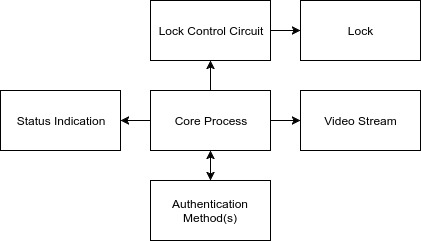
\includegraphics[width=\textwidth]{Diagrams/hardware_block}
	\caption{Hardware Block Diagram}
	\label{fig:hardware-block}
\end{figure}

%---------------------------------------------------------------------------------

\subsection{Core Software}



%---------------------------------------------------------------------------------

\subsection{Authentication Modules}

To meet the requirement of having a modular framework that supports multiple authentication methods, modules that 
perform the gathering of authentication data can be attached to the system, to increase the authentication options. As 
a result, multiple design patterns emerged immediately in the design of the software for the modules. Interfacing with 
the system core woud be the same across all authentication modules, so only the method used to gather authentication 
data is unique to each module. Two design patterns can be extracted from this statement: an Adapter pattern, where the 
Adaptee provides the interfaces necessary for communicating with the core, and a Template method for handling the 
authentication data. The Adapter can simply implement the Template method, as well as add any other functionality 
necessary for the means of authentication.

Talk about actors-boundaries-controllers-entities here

In the planning stages of the project, it was intended that the authentication modules would communicate with a central 
single-board microcontroller, such as a Arduino, which would be deemed a "communication board." This communication board
would be responsible for receiving data from the authentication modules, and for error detection and error correction, 
removing that overhead from the central computer. Once all of the authentication data was gathered, the board would send 
the data over a USB connection to the central computer. However, this design was tossed, for multiple reasons:
\begin{enumerate}
    \item The Arduino, as well as most other microcontrollers in the hobby market, can only communicate with another 
    Arduino over I2C;
    \item There is only one pair of pins reserved for I2C on most microcontrollers, meaning there can only be one 
    "slave" for each "master" communication board (refer to pinout here);
    \item Connecting all of the authentication modules over USB allowed for far more modularity than the "communication
    board" would have.
\end{enumerate}

Maybe add a figure of the Arduino pinout here?

Thus, the idea of using I2C communcation was scrapped, in favour of simply connecting each module to the core over USB. 
This simplified the development of communication modules considerably.


%=================================================================================

\section{Cloud}

%=================================================================================

% For the physical thing - not sure if this should be here since Michel et al did basically all of this ;)
\section{Lock Demonstration}

This chapter will be about the design and construction of the demo unit used at the poster fair

%=================================================================================

\chapter{System Implementation}

%=================================================================================

\section{Android}

The Android application was developed using Android Studio exclusively, and is primarily composed of Java classes, XML
documents, and gradle build files. Android studio was selected since it seemed to be the natural tool for writing an
Android application, and didn't have any negatives with respect to our requirements. Gradle was chosen as the build
tool as it is naturally integrated with Android studio.

\subsection{Server Interfacing}

Connections to the server were managed through the android Volley API. Volley provides a simple interface over which
HTTP and HTTPS messages can be sent. Standard operation of Volley follows a simple procedure: first a RequestQueue is
set up, and then various Requests are enqueued. These requests are then dequeued by the RequestQueue's thread, which
then creates an HTTP/HTTPS connection. The response that comes back over the connection is handled by another thread.

The code for handling these responses is put in a class that extends a Response.Listener of a given type. Since these
classes have just a few relatively simple methods, anonymous classes were used in all cases. Further, we decided that
handling the parsing shoudl be done as safely as possible, so all responses were first parsed simply as Strings. Then,
the response was attempted to be parsed as a JSON object of the type expected from the server. If that parsing failed,
the message was instead considered a error, and handled from there.

\subsection{HMAC}

Since the server used HMAC to handle security issues, the application needed to make frequent use of the headers that
the server expected to handle authentication. For this reason, a helper class called HMACHelper, was created. This
class provided methods that were commonly used by all requests about data particular to the current user. Most notably,
HMACHelper provided a method which calculated the secret using the same algorithm that the server would use. To
reiterate how HMAC functions, the body of the message is hashed using a private key shared by the server with the
application. When the application sends data that requires authentication, the server checks that the secret value
provided by the application matches what it calculates using the body of the message as well as the private key
associated with the user. These private keys are generated by the server when the user logs in to the application,
and expire over time, creating the notion of a session.

The precise algorithm used for the hashing function matches the decision made for the server. This is necessary, since
otherwise the secret values would not match between the application and the server. The application relies on a version
of the Password-Based Key Derivation Function algorithm using SHA256 to be available on the Android device. The only
workaround for this added requirement would have been to implement the algorithm (specified in RFC 2898 with test
vectors in RFC 6070) ourselves, however doing so is known to be quite dangerous as any minor error could result in a
security breach. In addition, the number of iterations and the resulting length also had to be kept as the same value.

%=================================================================================

\section{Hardware}

The hardware portion of the project consisted of two major portions: the 

Since driving the LEDs and the electrical lock only requires digital output, no analog pins would be necessary. While 
the single-board microcontrollers considered had optional boards which could add Wifi or Ethernet capabilities, they 
would not have been a sufficient solution to run the core process, as they were lacking a sufficient number of USB 
ports, and the overhead for implementing the core would have been too high. Because the microcontrollers do not run an 
operating system, 

A Raspberry Pi was ultimately selected as the computer to run the core process. The Pi 3 Model B has four USB ports, 
built-in Wifi capability, and forty pins for general-purpose IO (GPIO). These hardware features made the Raspberry Pi the best 
out-of-the-box solution to run the core process.

\subsection{Lock Control Circuit}

The next design problem to consider was the means to control the status of the electric lock. The simplest locks 
available, solenoid locks and electric strike locks, do not include any control mechanisms. They are either powered on, 
to disengage the lock, or powered off and locked. Therefore, it was necessary to implement a circuit to control the power to the 
lock, with the switching being driven by one of the Raspberry Pi's GPIO pins. There were two options considered for 
this:

1- Transistor/diode circuit

This circuit would use a TIP120 Darlington transistor, coupled with a 1N4004 flyback diode, to drive the lock. The circuit is 
demonstrated in figure NEXT.

Figure of circuit

Some heat-related math for the transistor:
The power law for a single voltage drop is $ P = IV = I^2R $. A transistor can be treated as two voltage drops, one 
from base to emitter ($ V_{BE} $), and another from collector to emitter ($ V_{CE} $), resulting in the power dissipated
by a transistor being given by:
$$ P = V_{BE}I_B + V_{CE}I_C $$
Since $ I_B \ll I_C $ when the lock circuit is active, the $ V_{BE}I_B $ term is negligible in this case, so the power
dissipated by the transistor is given by:
$$ P = V_{CE}I_C $$
At steady state, the voltage drop from the solenoid is negligible, as $ \frac{di}{dt} $ is zero, resulting in $ V = 
L\frac{di}{dt} = 0 $. This means that the voltage drop across the transistor, from emitter to collector, is 12V. Given
that the solenoid draws $\SI{650}{\milli\ampere}$ of current, the power across the transistor is:
$$ P = \SI{12}{\volt} \times \SI{650}{\milli\ampere} $$
$$ P = \SI{7.8}{\watt} $$
This power dissipation is quite significant in comparison to, for example, the resistors in the LED circuit, which at 
most will dissipate about $\SI{50}{\milli\watt}$. (n.b. should I put the math behind this in an appendix?) A heat 
dissipation mechanism would be necessary to ensure that the system does not heat up dangerously while in operation, 
which may not be practical in a real-life scenario. Secure systems should be completely enclosed, as a fan would 
introduce a point of physical access to the system.

Insert some more math and talk about the flyback diode to deal with the voltage spike - take the lock to a DOE lab at 
some point and measure the voltage spike when 12V DC is applied, to see what the minimum RB breakdown voltage should be

2- Relay circuit

Internally, a relay is very similar to the transistor/diode circuit, with a mechanical switch added. The relay itself 
has three inputs, and three outputs. The inputs are a positive voltage ($ V_{CC} $), ground (GND), and an input signal 
(IN). The outputs are a normally-closed terminal (NC), a common terminal (CO), and a normally-open terminal (NO). The 
circuit diagram of a relay is shown in Figure~\ref{fig:relay-circuit-diagram}.

\begin{figure}
	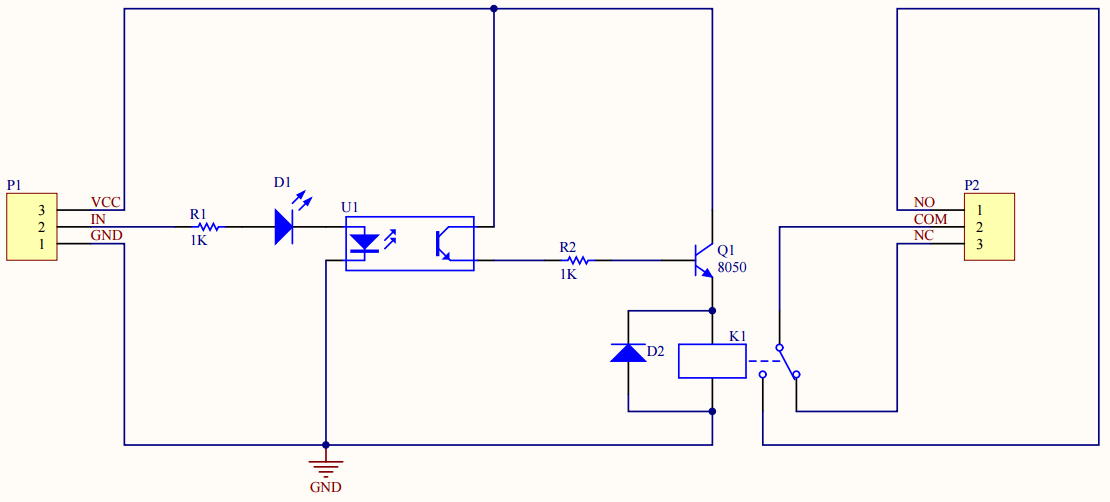
\includegraphics[width=\textwidth]{Diagrams/relay_circuit}
	\caption{Relay Circuit Diagram~\autocite{RELAYCIRCUIT}}
	\label{fig:relay-circuit-diagram}
\end{figure}

What separates the relay from a transistor/diode circuit is that it uses a solenoid internally to flip a mechanical 
switch. When the IN signal is low (0 volts), the switch short-circuits the "normally closed" connection, allowing
current to flow from the NC terminal to the CO terminal. The NO terminal is open-circuited, so no current will flow.
When the IN signal is high (5 volts), the solenoid inside the relay generates a magnetic field, which causes the switch 
to instead short-circuit the "normally open" connection, allowing current to flow from the NO terminal to the CO 
terminal, while the NC terminal is open-circuited. 

\subsection{Lock Control Software}

\subsection{Authentication Modules}

%=================================================================================

\section{Cloud}

%=================================================================================

\chapter{Testing and Bug Fixes}

% Not really sure what to go with here

%=================================================================================

\chapter{Conclusions}

%=================================================================================   

\appendix

%=================================================================================

\chapter{Sample Appendix}

%=================================================================================

\addcontentsline{toc}{chapter}{Bibliography} % Need this so it appears in the ToC
\printbibliography

\end{document}
